\documentclass[12pt]{article}

\usepackage{sbc-template}
\usepackage[utf8]{inputenc}
\usepackage[T1]{fontenc}
\usepackage[english,brazilian]{babel}
\usepackage{graphicx,url}
\usepackage{booktabs}
\usepackage{array}
\usepackage{amsmath}

\sloppy

% Relatório da parte 5 (K-means). O relatório da parte 4 (SVM) é o main.tex, na mesma pasta.
% Números gerados por scripts/clusters_report.py (numeros_clusters) e, para a curadoria da base,
% por scripts/svm_report.py (numeros_svm).
% Gerado por scripts/svm_report.py a partir de report/results/svm_dados.json; não editar.
\newcommand{\svLinhasBrutas}{32.561}
\newcommand{\svPositivosBrutos}{24,1}
\newcommand{\svDuplicadas}{24}
\newcommand{\svAusentes}{2.398}
\newcommand{\svPositivosAusentes}{13,9}
\newcommand{\svLinhas}{30.139}
\newcommand{\svLinhasEn}{30,139}
\newcommand{\svPositivos}{24,9}
\newcommand{\svNPositivos}{7.506}
\newcommand{\svPiso}{75,1}
\newcommand{\svPisoEn}{75.1}
\newcommand{\svRazaoClasses}{3,0}
\newcommand{\svColunas}{80}
\newcommand{\svCorrFnlwgt}{$-$0,009}
\newcommand{\svPerfisConflito}{673}
\newcommand{\svLinhasConflito}{2.404}
\newcommand{\svPctConflito}{8}
\newcommand{\svErrosIrred}{867}
\newcommand{\svIrredPct}{2,9}
\newcommand{\svTeto}{97,1}
\newcommand{\svTetoEn}{97.1}
\newcommand{\svRepetemPerfil}{5.057}
\newcommand{\svCasados}{45,5}
\newcommand{\svNuncaCasou}{4,8}
\newcommand{\svEstudoNove}{16,4}
\newcommand{\svEstudoTreze}{42,2}
\newcommand{\svEstudoQuinze}{74,9}
\newcommand{\svCorrEstudo}{0,34}
\newcommand{\svCorrIdade}{0,24}
\newcommand{\svCorrHoras}{0,23}
\newcommand{\svCorrGanho}{0,22}
\newcommand{\svCorrPerda}{0,15}
\newcommand{\svGanhoMax}{99.999}
\newcommand{\svTreino}{24.111}
\newcommand{\svTeste}{6.028}
\newcommand{\svPositivosTeste}{1.501}
\newcommand{\svMargem}{30,4}
\newcommand{\svVetNeg}{4.232}
\newcommand{\svVetPos}{3.999}
\newcommand{\svKLinSVC}{84,6}
\newcommand{\svKSVCLin}{84,5}
\newcommand{\svKPoliDois}{85,0}
\newcommand{\svKPoliTres}{85,1}
\newcommand{\svKRBF}{84,9}
\newcommand{\svKAucLinSVC}{89,8}
\newcommand{\svKAucRBF}{89,1}
\newcommand{\svRazaoLinear}{59}
\newcommand{\svPadCom}{85,0}
\newcommand{\svPadSem}{80,6}
\newcommand{\svPadFCom}{67,6}
\newcommand{\svPadFSem}{50,8}
\newcommand{\svPadVetSem}{16.995}
\newcommand{\svPadVetSemPct}{70}
\newcommand{\svPadTempoSem}{29}
\newcommand{\svPadTempoCom}{6,6}
\newcommand{\svLinPadCom}{84,6}
\newcommand{\svLinPadSem}{84,6}
\newcommand{\svMapaMelhor}{85,45}
\newcommand{\svMapaMelhorC}{1}
\newcommand{\svMapaMelhorG}{0,3}
\newcommand{\svMapaPerto}{13}
\newcommand{\svMapaComb}{35}
\newcommand{\svMapaCanto}{75,1}
\newcommand{\svGammaUmTreino}{90,5}
\newcommand{\svGammaUmVal}{83,5}
\newcommand{\svMapaTempoMax}{41,6}
\newcommand{\svInclSVC}{1,93}
\newcommand{\svInclSVCLin}{1,95}
\newcommand{\svInclLinSVC}{1,05}
\newcommand{\svTempoSVC}{5,8}
\newcommand{\svTempoLinSVC}{0,07}
\newcommand{\svGTresAuc}{88,0}
\newcommand{\svGUmAuc}{89,7}
\newcommand{\svGTresAcc}{85,2}
\newcommand{\svGUmAcc}{85,5}
\newcommand{\svGTresSeeds}{5}
\newcommand{\svGUmSeeds}{4}
\newcommand{\svGTresVet}{9.232}
\newcommand{\svGUmVet}{8.340}
\newcommand{\svLinC}{0,1}
\newcommand{\svLinCSeeds}{7}
\newcommand{\svRBFCUmSeeds}{9}
\newcommand{\svPoliSeeds}{9}
\newcommand{\svArvComb}{8}
\newcommand{\svRedeComb}{10}
\newcommand{\svRedeEpMin}{33}
\newcommand{\svRedeEpMax}{86}
\newcommand{\svBuscaTotalRBF}{82}
\newcommand{\svBuscaTotalSVM}{104}
\newcommand{\svBuscaTotalRede}{17}
\newcommand{\svRecallRBF}{61}
\newcommand{\svRecallPesos}{85}
\newcommand{\svRBFPrevS}{2,0}
\newcommand{\svRazaoPrevRBFLin}{448}
\newcommand{\svRazaoPrevRBFRede}{361}
\newcommand{\svMajAcc}{75,1}
\newcommand{\svMajAccEn}{75.1}
\newcommand{\svMajSd}{0,0}
\newcommand{\svMajFum}{42,9}
\newcommand{\svMajFpos}{0,0}
\newcommand{\svMajAuc}{50,0}
\newcommand{\svMajAucEn}{50.0}
\newcommand{\svMajFP}{0}
\newcommand{\svMajFN}{1.501}
\newcommand{\svMajTreino}{0,01}
\newcommand{\svMajPrev}{4,3}
\newcommand{\svRegraAcc}{75,1}
\newcommand{\svRegraAccEn}{75.1}
\newcommand{\svRegraSd}{0,0}
\newcommand{\svRegraFum}{42,9}
\newcommand{\svRegraFpos}{0,0}
\newcommand{\svRegraAuc}{75,6}
\newcommand{\svRegraAucEn}{75.6}
\newcommand{\svRegraFP}{0}
\newcommand{\svRegraFN}{1.501}
\newcommand{\svRegraTreino}{0,02}
\newcommand{\svRegraPrev}{4,8}
\newcommand{\svLogAcc}{84,8}
\newcommand{\svLogAccEn}{84.8}
\newcommand{\svLogSd}{0,3}
\newcommand{\svLogFum}{78,3}
\newcommand{\svLogFpos}{66,5}
\newcommand{\svLogAuc}{90,2}
\newcommand{\svLogAucEn}{90.2}
\newcommand{\svLogFP}{325}
\newcommand{\svLogFN}{592}
\newcommand{\svLogTreino}{0,06}
\newcommand{\svLogPrev}{4,5}
\newcommand{\svArvAcc}{85,2}
\newcommand{\svArvAccEn}{85.2}
\newcommand{\svArvSd}{0,4}
\newcommand{\svArvFum}{78,4}
\newcommand{\svArvFpos}{66,4}
\newcommand{\svArvAuc}{90,0}
\newcommand{\svArvAucEn}{90.0}
\newcommand{\svArvFP}{277}
\newcommand{\svArvFN}{617}
\newcommand{\svArvTreino}{0,06}
\newcommand{\svArvPrev}{5,1}
\newcommand{\svArvBusca}{7,3}
\newcommand{\svRFAcc}{84,3}
\newcommand{\svRFAccEn}{84.3}
\newcommand{\svRFSd}{0,4}
\newcommand{\svRFFum}{78,1}
\newcommand{\svRFFpos}{66,5}
\newcommand{\svRFAuc}{89,1}
\newcommand{\svRFAucEn}{89.1}
\newcommand{\svRFFP}{391}
\newcommand{\svRFFN}{559}
\newcommand{\svRFTreino}{2,8}
\newcommand{\svRFPrev}{180}
\newcommand{\svLinAcc}{84,8}
\newcommand{\svLinAccEn}{84.8}
\newcommand{\svLinSd}{0,3}
\newcommand{\svLinFum}{78,2}
\newcommand{\svLinFpos}{66,2}
\newcommand{\svLinAuc}{90,2}
\newcommand{\svLinAucEn}{90.2}
\newcommand{\svLinFP}{311}
\newcommand{\svLinFN}{604}
\newcommand{\svLinTreino}{0,05}
\newcommand{\svLinPrev}{4,5}
\newcommand{\svLinBusca}{1,2}
\newcommand{\svRBFAcc}{85,4}
\newcommand{\svRBFAccEn}{85.4}
\newcommand{\svRBFSd}{0,4}
\newcommand{\svRBFFum}{79,0}
\newcommand{\svRBFFpos}{67,5}
\newcommand{\svRBFAuc}{88,9}
\newcommand{\svRBFAucEn}{88.9}
\newcommand{\svRBFFP}{294}
\newcommand{\svRBFFN}{587}
\newcommand{\svRBFTreino}{5,7}
\newcommand{\svRBFPrev}{2016}
\newcommand{\svRBFBusca}{8,0}
\newcommand{\svRBFVet}{8.764}
\newcommand{\svPoliAcc}{85,2}
\newcommand{\svPoliAccEn}{85.2}
\newcommand{\svPoliSd}{0,4}
\newcommand{\svPoliFum}{78,7}
\newcommand{\svPoliFpos}{66,9}
\newcommand{\svPoliAuc}{90,2}
\newcommand{\svPoliAucEn}{90.2}
\newcommand{\svPoliFP}{298}
\newcommand{\svPoliFN}{596}
\newcommand{\svPoliTreino}{3,6}
\newcommand{\svPoliPrev}{488}
\newcommand{\svPoliBusca}{2,2}
\newcommand{\svPoliVet}{8.128}
\newcommand{\svPesosAcc}{80,9}
\newcommand{\svPesosAccEn}{80.9}
\newcommand{\svPesosSd}{0,3}
\newcommand{\svPesosFum}{77,6}
\newcommand{\svPesosFpos}{69,0}
\newcommand{\svPesosAuc}{89,8}
\newcommand{\svPesosAucEn}{89.8}
\newcommand{\svPesosFP}{929}
\newcommand{\svPesosFN}{221}
\newcommand{\svPesosTreino}{6,3}
\newcommand{\svPesosPrev}{2283}
\newcommand{\svPesosVet}{9.995}
\newcommand{\svRedeAcc}{85,2}
\newcommand{\svRedeAccEn}{85.2}
\newcommand{\svRedeSd}{0,6}
\newcommand{\svRedeFum}{79,4}
\newcommand{\svRedeFpos}{68,4}
\newcommand{\svRedeAuc}{90,8}
\newcommand{\svRedeAucEn}{90.8}
\newcommand{\svRedeFP}{362}
\newcommand{\svRedeFN}{533}
\newcommand{\svRedeTreino}{1,0}
\newcommand{\svRedePrev}{5,6}
\newcommand{\svRedeBusca}{1,7}
\newcommand{\svDifRBFLinAcc}{+0,57}
\newcommand{\svSeedsRBFLinAcc}{10}
\newcommand{\svPRBFLinAcc}{0,002}
\newcommand{\svDifRBFLinFum}{+0,82}
\newcommand{\svSeedsRBFLinFum}{10}
\newcommand{\svPRBFLinFum}{0,002}
\newcommand{\svDifRBFLinAuc}{$-$1,31}
\newcommand{\svSeedsRBFLinAuc}{0}
\newcommand{\svPRBFLinAuc}{0,002}
\newcommand{\svDifRBFRFAcc}{+1,14}
\newcommand{\svSeedsRBFRFAcc}{10}
\newcommand{\svPRBFRFAcc}{0,002}
\newcommand{\svDifRBFRFFum}{+0,93}
\newcommand{\svSeedsRBFRFFum}{10}
\newcommand{\svPRBFRFFum}{0,002}
\newcommand{\svDifRBFRFAuc}{$-$0,25}
\newcommand{\svSeedsRBFRFAuc}{5}
\newcommand{\svPRBFRFAuc}{0,322}
\newcommand{\svDifRBFArvAcc}{+0,22}
\newcommand{\svSeedsRBFArvAcc}{6}
\newcommand{\svPRBFArvAcc}{0,160}
\newcommand{\svDifRBFArvFum}{+0,61}
\newcommand{\svSeedsRBFArvFum}{8}
\newcommand{\svPRBFArvFum}{0,037}
\newcommand{\svDifRBFArvAuc}{$-$1,09}
\newcommand{\svSeedsRBFArvAuc}{0}
\newcommand{\svPRBFArvAuc}{0,002}
\newcommand{\svDifPoliRBFAcc}{$-$0,23}
\newcommand{\svSeedsPoliRBFAcc}{2}
\newcommand{\svPPoliRBFAcc}{0,014}
\newcommand{\svDifPoliRBFFum}{$-$0,36}
\newcommand{\svSeedsPoliRBFFum}{1}
\newcommand{\svPPoliRBFFum}{0,006}
\newcommand{\svDifPoliRBFAuc}{+1,34}
\newcommand{\svSeedsPoliRBFAuc}{10}
\newcommand{\svPPoliRBFAuc}{0,002}
\newcommand{\svDifLinLogAcc}{+0,02}
\newcommand{\svSeedsLinLogAcc}{7}
\newcommand{\svPLinLogAcc}{0,369}
\newcommand{\svDifLinLogFum}{$-$0,13}
\newcommand{\svSeedsLinLogFum}{1}
\newcommand{\svPLinLogFum}{0,006}
\newcommand{\svDifLinLogAuc}{$-$0,02}
\newcommand{\svSeedsLinLogAuc}{3}
\newcommand{\svPLinLogAuc}{0,160}
\newcommand{\svDifRedeRBFAcc}{$-$0,22}
\newcommand{\svSeedsRedeRBFAcc}{2}
\newcommand{\svPRedeRBFAcc}{0,129}
\newcommand{\svDifRedeRBFFum}{+0,32}
\newcommand{\svSeedsRedeRBFFum}{7}
\newcommand{\svPRedeRBFFum}{0,105}
\newcommand{\svDifRedeRBFAuc}{+1,96}
\newcommand{\svSeedsRedeRBFAuc}{10}
\newcommand{\svPRedeRBFAuc}{0,002}
\newcommand{\svDifRedeLinAcc}{+0,35}
\newcommand{\svSeedsRedeLinAcc}{9}
\newcommand{\svPRedeLinAcc}{0,025}
\newcommand{\svDifRedeLinFum}{+1,14}
\newcommand{\svSeedsRedeLinFum}{10}
\newcommand{\svPRedeLinFum}{0,002}
\newcommand{\svDifRedeLinAuc}{+0,66}
\newcommand{\svSeedsRedeLinAuc}{10}
\newcommand{\svPRedeLinAuc}{0,002}
\newcommand{\svDifRedeArvAcc}{+-0,00}
\newcommand{\svSeedsRedeArvAcc}{5}
\newcommand{\svPRedeArvAcc}{0,941}
\newcommand{\svDifRedeArvFum}{+0,93}
\newcommand{\svSeedsRedeArvFum}{10}
\newcommand{\svPRedeArvFum}{0,002}
\newcommand{\svDifRedeArvAuc}{+0,88}
\newcommand{\svSeedsRedeArvAuc}{10}
\newcommand{\svPRedeArvAuc}{0,002}
\newcommand{\svDifRedePoliAcc}{+0,01}
\newcommand{\svSeedsRedePoliAcc}{5}
\newcommand{\svPRedePoliAcc}{1,000}
\newcommand{\svDifRedePoliFum}{+0,68}
\newcommand{\svSeedsRedePoliFum}{9}
\newcommand{\svPRedePoliFum}{0,010}
\newcommand{\svDifRedePoliAuc}{+0,62}
\newcommand{\svSeedsRedePoliAuc}{10}
\newcommand{\svPRedePoliAuc}{0,002}
\newcommand{\svDifRedeLogAcc}{+0,37}
\newcommand{\svSeedsRedeLogAcc}{9}
\newcommand{\svPRedeLogAcc}{0,027}
\newcommand{\svDifRedeLogFum}{+1,02}
\newcommand{\svSeedsRedeLogFum}{10}
\newcommand{\svPRedeLogFum}{0,002}
\newcommand{\svDifRedeLogAuc}{+0,64}
\newcommand{\svSeedsRedeLogAuc}{10}
\newcommand{\svPRedeLogAuc}{0,002}
\newcommand{\svDifRFArvAcc}{$-$0,92}
\newcommand{\svSeedsRFArvAcc}{0}
\newcommand{\svPRFArvAcc}{0,002}
\newcommand{\svDifRFArvFum}{$-$0,32}
\newcommand{\svSeedsRFArvFum}{3}
\newcommand{\svPRFArvFum}{0,232}
\newcommand{\svDifRFArvAuc}{$-$0,84}
\newcommand{\svSeedsRFArvAuc}{0}
\newcommand{\svPRFArvAuc}{0,002}
\newcommand{\svDifArvLogAcc}{+0,37}
\newcommand{\svSeedsArvLogAcc}{8}
\newcommand{\svPArvLogAcc}{0,019}
\newcommand{\svDifArvLogFum}{+0,09}
\newcommand{\svSeedsArvLogFum}{7}
\newcommand{\svPArvLogFum}{0,375}
\newcommand{\svDifArvLogAuc}{$-$0,24}
\newcommand{\svSeedsArvLogAuc}{2}
\newcommand{\svPArvLogAuc}{0,049}

% Gerado por scripts/clusters_report.py a partir de report/results/clusters_dados.json; não editar.
\newcommand{\clLinhas}{30.139}
\newcommand{\clColunas}{80}
\newcommand{\clPositivos}{24,9}
\newcommand{\clComGanho}{8,4}
\newcommand{\clComPerda}{4,7}
\newcommand{\clComCapital}{13}
\newcommand{\clTeto}{148}
\newcommand{\clTrocaAnos}{18,6}
\newcommand{\clDesvioIdade}{13,1}
\newcommand{\clParteTexto}{36,6}
\newcommand{\clParteNum}{63,4}
\newcommand{\clPartePais}{2,1}
\newcommand{\clParteOcup}{11,3}
\newcommand{\clParteUmNum}{12,7}
\newcommand{\clSemLogMax}{13,3}
\newcommand{\clComLogMax}{4,4}
\newcommand{\clComLogZero}{$-$0,30}
\newcommand{\clSemLogTetoGrupo}{148}
\newcommand{\clSemLogPerda}{1.394}
\newcommand{\clComLogGanho}{2.510}
\newcommand{\clComLogPerda}{1.427}
\newcommand{\clComLogGanhoPos}{63,5}
\newcommand{\clComLogPerdaPos}{51,6}
\newcommand{\clQuedaDoisTres}{28.411}
\newcommand{\clQuedaQuatroCinco}{15.082}
\newcommand{\clQuedaCincoSeis}{8.492}
\newcommand{\clQuedaSeisSete}{6.317}
\newcommand{\clSilDois}{0,31}
\newcommand{\clSilSeis}{0,17}
\newcommand{\clDbDois}{1,27}
\newcommand{\clDbSeis}{1,71}
\newcommand{\clAriDoisMin}{$-$0,05}
\newcommand{\clAriTres}{0,59}
\newcommand{\clAriCinco}{0,977}
\newcommand{\clAriSeis}{0,995}
\newcommand{\clAriOito}{0,997}
\newcommand{\clAriNove}{0,79}
\newcommand{\clAriSeisUm}{0,59}
\newcommand{\clPioraSeisUm}{3}
\newcommand{\clPioraMin}{1}
\newcommand{\clPioraMax}{6}
\newcommand{\clTempoSeis}{0,95}
\newcommand{\clTempoSeisUm}{0,11}
\newcommand{\clTempoDois}{0,20}
\newcommand{\clAjustes}{180}
\newcommand{\clPureza}{77,5}
\newcommand{\clChute}{75,1}
\newcommand{\clPurezaGanho}{2,4}
\newcommand{\clAriRenda}{0,09}
\newcommand{\clSvmAcc}{85,4}
\newcommand{\clVarUm}{19,5}
\newcommand{\clVarDois}{13,5}
\newcommand{\clVarTotal}{33}
\newcommand{\clMulheresBase}{32,4}
\newcommand{\clMulheresTres}{8,3}
\newcommand{\clMulheresUm}{47,7}
\newcommand{\clMulheresDois}{48,3}
\newcommand{\clNegrosBase}{9,3}
\newcommand{\clNegrosUm}{12,8}
\newcommand{\clNegrosDois}{13,4}
\newcommand{\clLinhasEn}{30,139}
\newcommand{\clPurezaEn}{77.5}
\newcommand{\clChuteEn}{75.1}
\newcommand{\clSvmAccEn}{85.4}
\newcommand{\clAriSeisEn}{0.995}
\newcommand{\clSilSeisEn}{0.17}
\newcommand{\clSemLogSilDois}{0,42}
\newcommand{\clSemLogSilSeis}{0,150}
\newcommand{\clComLogSilSeis}{0,165}
\newcommand{\clSemLogMenorDois}{1.393}
\newcommand{\clSemLogMenor}{148}
\newcommand{\clComLogMenor}{1.427}
\newcommand{\clComLogMenorDois}{2.533}
\newcommand{\clTempoMax}{1,3}
\newcommand{\clIterDois}{4}
\newcommand{\clIterDez}{51}
\newcommand{\clIterSeis}{46}
\newcommand{\clCasadosTres}{90}
\newcommand{\clMaridoTres}{84}
\newcommand{\clNuncaUm}{82}
\newcommand{\clFilhoUm}{45}
\newcommand{\clDivorcDois}{34}
\newcommand{\clViuvoDois}{11}
\newcommand{\clChefeDois}{23}
\newcommand{\clEspecQuatro}{40}
\newcommand{\clGerenQuatro}{25}
\newcommand{\clSilGUm}{0,19}
\newcommand{\clSilNegGUm}{1}
\newcommand{\clSilGDois}{0,06}
\newcommand{\clSilNegGDois}{28}
\newcommand{\clSilGTres}{0,17}
\newcommand{\clSilNegGTres}{0}
\newcommand{\clSilGQuatro}{0,10}
\newcommand{\clSilNegGQuatro}{7}
\newcommand{\clSilGCinco}{0,40}
\newcommand{\clSilNegGCinco}{0}
\newcommand{\clSilGSeis}{0,30}
\newcommand{\clSilNegGSeis}{0}
\newcommand{\clPosUm}{1,1}
\newcommand{\clPessoasUm}{8.439}
\newcommand{\clPosUmEn}{1.1}
\newcommand{\clPosDois}{12,6}
\newcommand{\clPessoasDois}{5.443}
\newcommand{\clPosDoisEn}{12.6}
\newcommand{\clPosTres}{27,5}
\newcommand{\clPessoasTres}{6.538}
\newcommand{\clPosTresEn}{27.5}
\newcommand{\clPosQuatro}{44,8}
\newcommand{\clPessoasQuatro}{5.791}
\newcommand{\clPosQuatroEn}{44.8}
\newcommand{\clPosCinco}{51,6}
\newcommand{\clPessoasCinco}{1.427}
\newcommand{\clPosCincoEn}{51.6}
\newcommand{\clPosSeis}{63,8}
\newcommand{\clPessoasSeis}{2.501}
\newcommand{\clPosSeisEn}{63.8}


\title{K-means na base Adult: que grupos de pessoas existem quando não olhamos a renda}

\author{Bernan R. do Nascimento\inst{1}, Paulo E. R. Araujo\inst{1}, Thiago R. P. de Carvalho\inst{1}}

\address{Universidade Federal do Piauí (UFPI)\\
  Programa de Pós-Graduação em Ciência da Computação -- Teresina -- PI -- Brasil\\
  PPGCC010 -- Aprendizagem de Máquina (2026.2) -- Prof. Vinicius Ponte Machado
  \email{bernanr7@gmail.com, pauloaraujo@ufpi.edu.br}
  \email{thiago.rafael.pc@gmail.com}
}

\begin{document}

\maketitle

\begin{abstract}
  We cluster \clLinhasEn{} people of the 1994 US census (Adult dataset) with K-means, an unsupervised
  method, using 10 attributes and leaving their income out, to find which groups of similar people make
  up the data. The preprocessing decides the groups: with one-hot encoding, a different occupation sets two
  people as far apart as about 19 years of age, and a logarithm on capital gain and loss removes an
  artificial group of \clTeto{} people at the census cap but makes the people with any capital form two
  groups of their own. With $k = 6$, chosen by the elbow and by stability across 10 seeds (ARI
  \clAriSeisEn), four groups differ by stage of life and type of work and two by capital. A silhouette of
  \clSilSeisEn{} shows no sharp groups. The groups follow income without having seen it, from \clPosUmEn\%
  to \clPosSeisEn\% above 50 thousand, but as predictors they are weak: a purity of \clPurezaEn\% against
  \clChuteEn\% for always answering ``no'' and \clSvmAccEn\% for a support vector machine trained on income.
\end{abstract}

\begin{resumo}
  Agrupamos \clLinhas{} pessoas do censo dos EUA de 1994 (base Adult) com o K-means, um método não
  supervisionado, a partir de 10 atributos e sem a renda, para descobrir que grupos de pessoas parecidas
  compõem a base. O pré-processamento decide os grupos: com o one-hot, trocar de ocupação afasta duas
  pessoas tanto quanto \clTrocaAnos{} anos de idade, e um logaritmo no ganho e na perda de capital tira um
  grupo artificial de \clTeto{} pessoas no teto do censo, mas faz quem tem capital formar dois grupos
  próprios. Com $k = 6$, escolhido pelo cotovelo e pela estabilidade entre 10 seeds (ARI de \clAriSeis),
  quatro grupos se distinguem pela fase da vida e pelo tipo de trabalho, e dois pelo capital. A silhueta de
  \clSilSeis{} mostra que não há grupos nítidos. Os grupos se ordenam pela renda sem tê-la visto, de
  \clPosUm\% a \clPosSeis\% acima de 50 mil, mas como previsão são fracos: pureza de \clPureza\%, contra
  \clChute\% de responder sempre ``não'' e \clSvmAcc\% de uma máquina de vetores de suporte treinada com a
  renda.
\end{resumo}

\section{Introdução}

A base Adult~\cite{uci:adult,kohavi:96} reúne cerca de 30 mil pessoas do censo dos EUA de 1994, cada uma descrita por 10 atributos, como idade, anos de estudo, estado civil e ocupação, e pela informação de a sua renda anual passar ou não de 50 mil dólares. Na parte anterior do trabalho, usamos essa base para prever a renda. Aqui a pergunta muda: em vez de prever, queremos descobrir que grupos de pessoas parecidas compõem a base.

Para isso, usamos o K-means~\cite{lloyd:82,macqueen:67}, um método não supervisionado. Os métodos supervisionados aprendem a partir de exemplos com a resposta; o K-means recebe só os atributos, sem a renda, e divide as pessoas em grupos de acordo com a distância entre elas. Não há resposta certa a acertar: avaliamos os grupos pela sua compacidade, pela sua estabilidade e pelo sentido que fazem. A renda entra só no fim, para conferir se os grupos encontrados têm relação com ela.

As contribuições são:
\begin{itemize}
  \item a medida do efeito do pré-processamento sobre os grupos: quanto cada atributo pesa na distância com o one-hot, e como o logaritmo no capital tira um grupo artificial mas faz quem tem capital formar grupos próprios (Seções~\ref{sec:cl_onehot} e~\ref{sec:cl_log});
  \item a escolha do número de grupos por métricas internas e pela estabilidade entre 10 seeds, que mostra por que o K-means precisa de várias inicializações (Seção~\ref{sec:cl_k});
  \item seis perfis de pessoas, descritos pela composição e pela coesão de cada grupo, que se ordenam pela renda sem tê-la visto, mas que, como previsão, ficam pouco acima do chute (Seções~\ref{sec:cl_grupos} e~\ref{sec:cl_renda}).
\end{itemize}

\section{Fundamentação}

\textbf{K-means.} O K-means~\cite{lloyd:82,macqueen:67} divide $n$ exemplos em $k$ grupos, com $k$ escolhido por quem o usa. Cada grupo é representado por um centro $\mu_j$, a média dos seus exemplos, e o algoritmo busca a partição de menor \emph{inércia}, a soma das distâncias ao quadrado de cada exemplo ao centro do seu grupo:
\begin{equation*}
  \text{inércia} = \sum_{i=1}^{n} \lVert x_i - \mu_{c(i)} \rVert^2 ,
\end{equation*}
em que $c(i)$ é o grupo do exemplo $i$. O algoritmo de Lloyd começa com $k$ centros e alterna dois passos até a partição parar de mudar: cada exemplo vai para o centro mais próximo, e cada centro passa a ser a média dos exemplos do seu grupo. Nenhum dos passos aumenta a inércia, de modo que o algoritmo sempre para, mas num mínimo local, que depende dos centros iniciais. O k-means++~\cite{arthur:07} sorteia esses centros dando mais chance a exemplos longe dos já escolhidos, o que espalha os centros pelo espaço, e é comum repetir o algoritmo com vários sorteios e ficar com a partição de menor inércia. Cada iteração custa proporcionalmente ao número de exemplos, ao número de grupos e ao número de atributos, e o custo total cresce linearmente com a base. Como mede distâncias a um centro, o K-means favorece grupos arredondados e de tamanho parecido.

\textbf{Distância e escala.} Como tudo depende da distância, atributos em escalas diferentes precisam ser postos numa escala comum, ou o de maior amplitude domina. A \emph{padronização} (z-score) transforma cada valor em $(x - \bar{x})/s$, de modo que o atributo fique com média 0 e desvio padrão 1, e a escala vem de todos os valores. A \emph{normalização} (min-max) transforma cada valor em $(x - \min)/(\max - \min)$, levando o atributo para o intervalo de 0 a 1, e a escala vem só dos dois extremos: um valor muito alto comprime todos os outros perto de zero. Usamos a padronização. Atributos de texto não têm distância natural; o \emph{one-hot} cria uma coluna de 0 ou 1 para cada categoria, e duas pessoas com categorias diferentes passam a diferir em duas colunas.

\textbf{Avaliação de agrupamentos.} Sem rótulos, a qualidade de uma partição é medida por índices internos. A inércia sempre cai quando $k$ aumenta, e por isso se procura o ``cotovelo'', o $k$ a partir do qual ela cai pouco. A silhueta~\cite{rousseeuw:87} de um exemplo compara a distância média $a$ aos exemplos do próprio grupo com a distância média $b$ aos do grupo vizinho mais próximo, $(b - a)/\max(a, b)$: vai de $-1$ a 1, e a média sobre os exemplos é maior para grupos compactos e separados. O índice de Davies-Bouldin~\cite{davies:79} toma, para cada grupo, a pior razão entre a soma dos espalhamentos de dois grupos e a distância entre os seus centros, e faz a média; quanto menor, melhor. Para comparar duas partições, como as de duas seeds ou a de um agrupamento e a dos rótulos, usamos o índice de Rand ajustado (ARI)~\cite{hubert:85}, que conta os pares de exemplos postos juntos ou separados nas duas partições, corrigido pelo acaso: vale 1 para partições idênticas e cerca de 0 para concordância casual, sem depender do número dado a cada grupo. A \emph{pureza} de uma partição em relação aos rótulos é a fração de exemplos que acertariam se cada grupo respondesse o rótulo mais comum entre os seus exemplos.

\textbf{Visualização.} A análise de componentes principais (PCA) encontra as direções em que os dados mais variam e projeta os exemplos nelas. Projetar em duas componentes permite desenhar grupos formados em muitas colunas, mas mostra só a parte da variação que essas duas direções explicam.

\section{Dados}\label{sec:km_dados}

A base Adult~\cite{uci:adult} foi extraída do censo dos EUA de 1994 e doada à UCI por Becker e Kohavi~\cite{kohavi:96}. A versão do Kaggle~\cite{kaggle:adult} tem \svLinhasBrutas{} registros, um por pessoa, com 14 atributos e o rótulo \texttt{income}, que diz se a renda anual passa de 50 mil dólares. A curadoria é a da parte anterior do trabalho: foram removidas \svDuplicadas{} linhas repetidas e \svAusentes{} com valor ausente (marcado com ``?''), e restam \svLinhas{} pessoas, \svPositivos\% com renda acima de 50 mil. Saíram também dois atributos: o \texttt{fnlwgt}, um peso amostral do censo, que não descreve a pessoa, e o \texttt{education}, que repete em texto os anos de estudo.

Ficam 10 atributos (Tabela~\ref{tab:km_atributos}): 5 numéricos e 5 de texto. Raça e sexo continuam no arquivo, mas ficam fora do agrupamento por decisão do grupo, como ficaram fora da classificação; são usados só depois, para ver como se distribuem nos grupos (Seção~\ref{sec:cl_sensiveis}). A renda também fica fora e serve só para comparar.

\begin{table}[ht]
\centering
\caption{Os 10 atributos usados no agrupamento, após a curadoria.}
\label{tab:km_atributos}
\footnotesize
\begin{tabular}{lll}
\toprule
Coluna original & Nome neste trabalho & Valores \\
\midrule
\texttt{age} & idade & 17 a 90 anos \\
\texttt{education.num} & anos de estudo & 1 a 16 \\
\texttt{capital.gain} & ganho de capital & 0 a \svGanhoMax{} dólares \\
\texttt{capital.loss} & perda de capital & 0 a 4.356 dólares \\
\texttt{hours.per.week} & horas por semana & 1 a 99 \\
\texttt{workclass} & classe de trabalho & 7 categorias \\
\texttt{marital.status} & estado civil & 7 categorias \\
\texttt{occupation} & ocupação & 14 categorias \\
\texttt{relationship} & relacionamento & 6 categorias \\
\texttt{native.country} & país de origem & 41 países \\
\bottomrule
\end{tabular}
\end{table}

Duas características da base pesam na distância entre as pessoas. O ganho e a perda de capital são zero para quase todos (só \clComGanho\% das pessoas têm algum ganho e \clComPerda\% alguma perda), com poucos valores muito altos: \clTeto{} pessoas têm ganho de 99.999 dólares, o teto do censo. E os atributos de texto são desequilibrados: 91\% das pessoas são dos EUA, enquanto a ocupação se divide em 14 categorias de tamanhos parecidos.

\section{Metodologia}\label{sec:km_metodo}

\textbf{Pré-processamento.} Usamos o mesmo pré-processamento da parte anterior do trabalho, em que treinamos máquinas de vetores de suporte (SVM)~\cite{cortes:95} para prever a renda: os 5 atributos numéricos padronizados e os 5 de texto em one-hot, num total de \clColunas{} colunas. A SVM com kernel RBF também mede distâncias, e o mesmo cuidado com a escala vale aqui. A única diferença é um logaritmo, $\log(1 + x)$, no ganho e na perda de capital antes da padronização; o ``1 +'' existe porque a maioria tem valor zero, e $\log 0$ não existe. A Seção~\ref{sec:cl_log} compara os grupos com e sem esse logaritmo.

\textbf{Protocolo.} Não há divisão em treino e teste, porque não há resposta a acertar: os grupos são formados na base inteira, e não há vazamento, porque a renda nunca entra no ajuste. Para cada $k$ de 2 a 10, o K-means roda com 10 seeds (0 a 9), e cada seed faz 10 inicializações com k-means++ e fica com a de menor inércia. A seed fixa o gerador de números aleatórios, e portanto quais centros iniciais são sorteados. Em cada ajuste, medimos a inércia, a silhueta e o índice de Davies-Bouldin. A silhueta compara todos os pares de pessoas e é calculada numa amostra fixa de 10 mil pessoas, a mesma em todos os ajustes. A estabilidade de cada $k$ é o ARI médio entre as partições das 10 seeds, comparadas duas a duas (45 pares), e repetimos o estudo com uma só inicialização por seed, para medir o que as 10 inicializações acrescentam.

\textbf{Partição descrita.} Escolhido o $k$, descrevemos a partição da seed 42, fora das seeds 0 a 9, como nas análises de uma seed das partes anteriores do trabalho. Não faz sentido tirar a média das 10 partições: o número que o K-means dá a cada grupo é arbitrário e muda de uma seed para outra. Para facilitar a leitura, os grupos foram renumerados de 1 a $k$ pelo percentual de renda alta; a renda só ordena os nomes, sem influenciar a formação dos grupos.

\textbf{Implementação.} Tudo foi feito com o scikit-learn~\cite{pedregosa:11}, e os tempos foram medidos num único núcleo de processador. O código, os resultados e o notebook com a análise completa estão no repositório do trabalho, na pasta \texttt{renda/}.

\section{Resultados}\label{sec:km_resultados}

\subsection{O efeito do one-hot na distância}\label{sec:cl_onehot}

O K-means agrupa pela distância euclidiana ao quadrado, que soma as diferenças coluna a coluna, de modo que o pré-processamento define o que é ``parecido''. Um atributo numérico padronizado contribui com o quadrado da diferença em desvios; um atributo de texto contribui com 0 quando duas pessoas têm a mesma categoria e com 2 quando têm categorias diferentes, porque uma coluna do one-hot apaga e outra acende, seja qual for o número de categorias. Assim, trocar de ocupação afasta duas pessoas tanto quanto \clTrocaAnos{} anos de diferença de idade ($\sqrt{2}$ desvios de \clDesvioIdade{} anos). Em média, porém, os atributos de texto pesam menos que os numéricos (Figura~\ref{fig:cl_peso}): para duas pessoas sorteadas, cada numérico contribui com 2, e cada atributo de texto com 2 vezes a chance de as duas terem categorias diferentes. Os 5 de texto respondem por \clParteTexto\% da distância média; o país, só por \clPartePais\%, porque 91\% das pessoas são dos EUA. A média esconde a forma: os numéricos variam aos poucos, e as categorias são degraus que tendem a marcar as fronteiras entre os grupos.

\begin{figure}[ht]
\centering
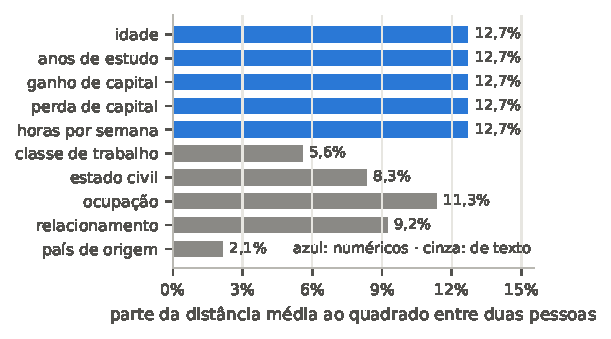
\includegraphics[width=.62\textwidth]{figures/clusters_peso.pdf}
\caption{Parte de cada atributo na distância média ao quadrado entre duas pessoas sorteadas (\clColunas{} colunas, com log no capital).}
\label{fig:cl_peso}
\end{figure}

\subsection{O efeito do logaritmo no capital}\label{sec:cl_log}

O ganho e a perda de capital são zero para quase todos: só \clComGanho\% das pessoas têm algum ganho e \clComPerda\% alguma perda, e poucos valores são muito altos. Padronizado sem log, o ganho de 99.999 dólares, o teto do censo, fica a \clSemLogMax{} desvios da média, e as \clTeto{} pessoas com esse valor formam um grupo só delas (Tabela~\ref{tab:cl_log}). Com o log, o máximo cai para \clComLogMax{} desvios e esse grupo desaparece. Surge, porém, outro efeito: quem não tem ganho fica em \clComLogZero{} desvio, e quem tem algum ganho fica perto de $+3$, um salto maior que qualquer troca de categoria. As \clComLogGanho{} pessoas com ganho e as \clComLogPerda{} com perda formam grupos próprios, com \clComLogGanhoPos\% e \clComLogPerdaPos\% acima de 50 mil. Mantivemos o log: esses dois grupos são reais e concentram a renda alta, enquanto o grupo das \clTeto{} pessoas é um artefato do teto do censo. A consequência é que, de $k = 4$ em diante, dois dos $k$ grupos ficam com os \clComCapital\% das pessoas que têm capital, e os demais dividem o resto.

\begin{table}[ht]
\centering
\caption{K-means com $k = 4$ e seed 42, sem e com log no ganho e na perda de capital.}
\label{tab:cl_log}
\footnotesize
\begin{tabular}{lrrrr}
\toprule
Grupo (k = 4, seed 42) & Pessoas & Com ganho (\%) & Com perda (\%) & $>$50K (\%) \\
\midrule
\multicolumn{5}{l}{\emph{Sem log}} \\
1º maior & 16.888 & 11,3 & 0,1 & 36,7 \\
2º maior & 11.709 & 4,1 & 0,1 & 3,7 \\
3º maior & 1.394 & 0,0 & 100,0 & 52,7 \\
4º maior & 148 & 100,0 & 0,0 & 100,0 \\
\midrule
\multicolumn{5}{l}{\emph{Com log}} \\
1º maior & 15.496 & 0,0 & 0,0 & 31,6 \\
2º maior & 10.706 & 0,3 & 0,0 & 2,6 \\
3º maior & 2.510 & 100,0 & 0,0 & 63,5 \\
4º maior & 1.427 & 0,0 & 100,0 & 51,6 \\
\bottomrule
\end{tabular}

\end{table}

A Figura~\ref{fig:cl_log} estende a comparação a todo $k$ de 2 a 10, na seed 42. Sem log, o menor grupo tem sempre \clSemLogMenor{} pessoas de $k = 4$ em diante: o grupo do teto do censo aparece em qualquer partição com quatro grupos ou mais, e a silhueta fica abaixo da versão com log (\clSemLogSilSeis{} contra \clComLogSilSeis{} em $k = 6$). A exceção é $k = 2$, em que a versão sem log tem silhueta maior (\clSemLogSilDois), porque separa só as \clSemLogMenorDois{} pessoas com perda de capital. Com log, o menor grupo passa a ser o das \clComLogMenor{} pessoas com perda, de $k = 3$ em diante: o logaritmo troca um grupo artificial por um grupo real.

\begin{figure}[ht]
\centering
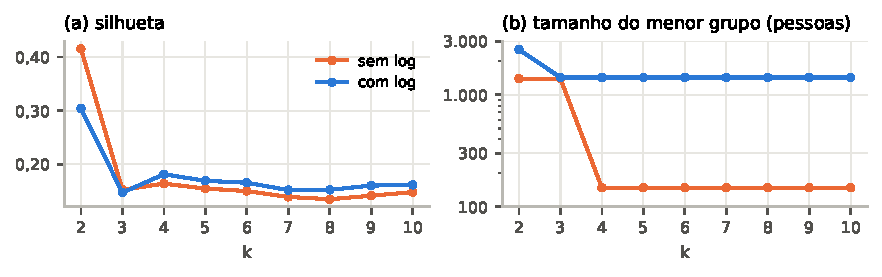
\includegraphics[width=\textwidth]{figures/clusters_log.pdf}
\caption{K-means sem e com log no capital, para $k$ de 2 a 10 (seed 42): silhueta e tamanho do menor grupo (escala logarítmica).}
\label{fig:cl_log}
\end{figure}

\subsection{Escolha do número de grupos}\label{sec:cl_k}

As métricas internas não apontam um $k$ claro (Figura~\ref{fig:cl_curvas} e Tabela~\ref{tab:cl_k}). Silhueta e Davies-Bouldin preferem $k = 2$ (\clSilDois{} e \clDbDois), mas esse $k$ só separa quem tem ganho de capital do resto: é a fronteira mais nítida da base, e diz pouco sobre as demais pessoas. Em 9 seeds o grupo pequeno é o do ganho; numa, o da perda, com quase a mesma inércia, o que explica o ARI mínimo de \clAriDoisMin{} entre seeds. De $k = 4$ em diante, as duas métricas ficam planas, com silhueta em torno de \clSilSeis. Valores tão baixos (acima de 0,5 indicariam grupos bem separados) mostram que a base não tem grupos nítidos: os grupos são regiões de uma nuvem contínua de pessoas. Na inércia, a queda de um $k$ para o seguinte passa de \clQuedaQuatroCinco{} (de 4 para 5) para \clQuedaCincoSeis{} (de 5 para 6) e \clQuedaSeisSete{} (de 6 para 7): o cotovelo fica entre 5 e 6.

\begin{figure}[ht]
\centering
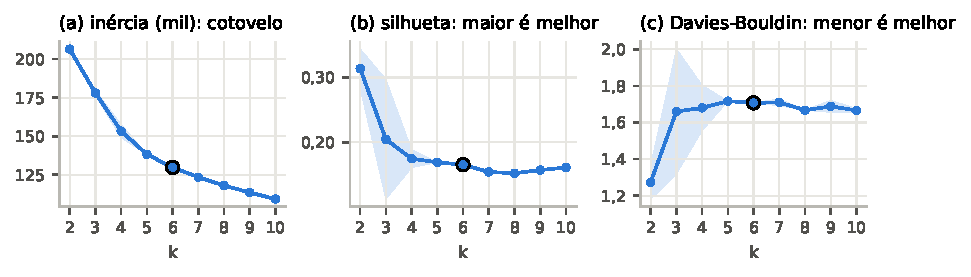
\includegraphics[width=\textwidth]{figures/clusters_curvas.pdf}
\caption{Métricas internas para $k$ de 2 a 10: média das 10 seeds (linha) e $\pm$ um desvio (faixa); o círculo marca $k = 6$.}
\label{fig:cl_curvas}
\end{figure}

\begin{table}[ht]
\centering
\caption{Métricas internas (média das 10 seeds) e estabilidade (ARI médio entre as seeds, 45 pares) por $k$.}
\label{tab:cl_k}
\footnotesize
\begin{tabular}{crrrrr}
\toprule
k & Inércia & Silhueta & Davies-Bouldin & ARI (10 inic.) & ARI (1 inic.) \\
\midrule
2 & 206.442 & 0,314 & 1,27 & 0,789 & 0,786 \\
3 & 178.031 & 0,204 & 1,66 & 0,589 & 0,605 \\
4 & 153.330 & 0,175 & 1,68 & 0,858 & 0,717 \\
5 & 138.247 & 0,169 & 1,72 & 0,977 & 0,856 \\
\textbf{6} & 129.755 & 0,165 & 1,71 & 0,995 & 0,588 \\
7 & 123.438 & 0,154 & 1,71 & 0,926 & 0,558 \\
8 & 118.019 & 0,152 & 1,67 & 0,997 & 0,566 \\
9 & 113.503 & 0,157 & 1,69 & 0,786 & 0,649 \\
10 & 109.249 & 0,161 & 1,67 & 0,904 & 0,730 \\
\bottomrule
\end{tabular}

\end{table}

Como as métricas empatam, a estabilidade desempata (Figura~\ref{fig:cl_estab}). Com 10 inicializações, as 10 seeds chegam praticamente à mesma partição em $k = 5$, 6 e 8 (ARI de \clAriCinco, \clAriSeis{} e \clAriOito), enquanto $k = 3$ (\clAriTres) e $k = 9$ (\clAriNove) são instáveis: o algoritmo corta uma região sem fronteira natural, e cada seed corta de um jeito. Com uma só inicialização por seed, cada sorteio para num mínimo local diferente: em $k = 6$, o ARI cai para \clAriSeisUm, e a inércia média piora entre \clPioraMin\% e \clPioraMax\% conforme o $k$. As 10 inicializações custam 10 vezes mais e compram a mesma resposta em todas as seeds.

\begin{figure}[ht]
\centering
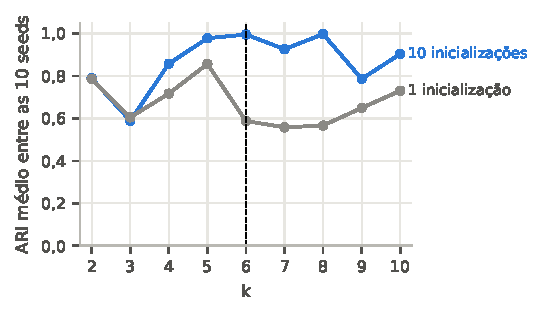
\includegraphics[width=.62\textwidth]{figures/clusters_estabilidade.pdf}
\caption{Estabilidade: ARI médio entre as partições das 10 seeds, com 10 inicializações por seed e com uma só.}
\label{fig:cl_estab}
\end{figure}

Escolhemos $k = 6$: está no cotovelo, é praticamente estável (ARI de \clAriSeis) e, como dois grupos ficam com o capital, deixa quatro grupos para quem não o tem. A Tabela~\ref{tab:cl_alt} mostra os dois vizinhos estáveis, $k = 5$ e $k = 8$, na seed 42. Os dois grupos do capital são os mesmos nos três $k$. Com $k = 5$, sobram três grupos sem capital: jovens solteiros, casados com pouco estudo e casados com muito estudo; os mais velhos sem cônjuge ficam diluídos entre os outros. Com $k = 8$, os jovens se dividem pelas horas de trabalho (22 anos e 20 horas por semana; 28 anos e 41 horas), surge um grupo de quem trabalha 66 horas por semana, e os mais velhos sem cônjuge continuam num grupo próprio, agora com 55 anos em média. O $k = 6$ é o menor $k$ que separa os mais velhos sem cônjuge dos casados, sem dividir os jovens por detalhes. A escolha combina métricas e interpretação, e $k = 5$ ou $k = 8$ também seriam defensáveis.

\begin{table}[ht]
\centering
\caption{As alternativas estáveis: perfis com $k = 5$ e $k = 8$ (seed 42), com os grupos ordenados pelo \% acima de 50 mil.}
\label{tab:cl_alt}
\scriptsize
\setlength{\tabcolsep}{3pt}
\begin{tabular}{clrrrrrlr}
\toprule
k & Grupo & Pessoas & Idade & \shortstack{Anos de\\estudo} & \shortstack{Horas por\\semana} & \shortstack{Casados\\(\%)} & Ocupação mais comum & \shortstack{$>$50K\\(\%)} \\
\midrule
5 & 1 & 9.282 & 25,9 & 9,6 & 34,9 & 7 & outros serviços & 1,8 \\
 & 2 & 9.313 & 47,6 & 8,5 & 38,9 & 61 & ofícios e reparos & 18,7 \\
 & 3 & 7.608 & 40,2 & 12,3 & 49,3 & 66 & especialista & 42,9 \\
 & 4 (todos com perda) & 1.427 & 41,6 & 11,0 & 43,5 & 64 & gerência & 51,6 \\
 & 5 (todos com ganho) & 2.509 & 43,8 & 11,1 & 44,2 & 68 & especialista & 63,6 \\
\midrule
8 & 1 & 2.551 & 22,9 & 9,2 & 20,3 & 6 & outros serviços & 1,1 \\
 & 2 & 7.403 & 28,5 & 9,8 & 41,1 & 1 & administrativo & 2,3 \\
 & 3 & 4.479 & 55,2 & 8,2 & 36,4 & 37 & administrativo & 11,6 \\
 & 4 & 5.344 & 37,5 & 9,0 & 41,9 & 100 & ofícios e reparos & 28,7 \\
 & 5 & 1.881 & 40,4 & 10,3 & 66,3 & 66 & gerência & 33,5 \\
 & 6 & 4.570 & 43,2 & 13,4 & 42,4 & 66 & especialista & 50,2 \\
 & 7 (todos com perda) & 1.427 & 41,6 & 11,0 & 43,5 & 64 & gerência & 51,6 \\
 & 8 (todos com ganho) & 2.484 & 43,7 & 11,2 & 44,2 & 68 & especialista & 64,1 \\
\bottomrule
\end{tabular}

\end{table}

\subsection{Os seis grupos}\label{sec:cl_grupos}

A partição da seed 42 coincide com as das seeds 0 a 9 (ARI entre 0,977 e 0,999 com cada uma). A Tabela~\ref{tab:cl_grupos} resume os grupos; os nomes são nossos, tirados do perfil médio, e o K-means devolve só um número por pessoa. Os grupos 1 a 4, sem capital, se separam pela fase da vida e pelo tipo de trabalho: jovens que nunca se casaram e muitas vezes moram com os pais (grupo 1); pessoas mais velhas, divorciadas ou viúvas, com pouco estudo (grupo 2); casados em ofícios manuais, com jornadas longas (grupo 3); e profissionais com muito estudo, especialistas e gerentes (grupo 4). Os grupos 5 e 6 são parecidos entre si nos demais atributos (cerca de 42 anos, 11 anos de estudo, dois terços casados): o que os separa do resto, e um do outro, é o capital.

\begin{table}[ht]
\centering
\caption{Perfil dos seis grupos ($k = 6$, seed 42): médias dos numéricos, \% de casados, a ocupação mais comum (com a sua parte no grupo) e \% acima de 50 mil.}
\label{tab:cl_grupos}
\scriptsize
\setlength{\tabcolsep}{3pt}
\begin{tabular}{lrrrrrlr}
\toprule
Grupo & Pessoas & Idade & \shortstack{Anos de\\estudo} & \shortstack{Horas por\\semana} & \shortstack{Casados\\(\%)} & Ocupação mais comum & \shortstack{$>$50K\\(\%)} \\
\midrule
1. Jovens solteiros & 8.439 & 25,7 & 9,4 & 34,4 & 3 & outros serviços (20\%) & 1,1 \\
2. Mais velhos sem cônjuge & 5.443 & 53,4 & 8,5 & 36,3 & 37 & administrativo (18\%) & 12,6 \\
3. Casados em ofícios manuais & 6.538 & 37,6 & 9,0 & 47,6 & 90 & ofícios e reparos (26\%) & 27,5 \\
4. Profissionais com muito estudo & 5.791 & 40,9 & 13,3 & 45,1 & 57 & especialista (40\%) & 44,8 \\
5. Com perda de capital & 1.427 & 41,6 & 11,0 & 43,5 & 64 & gerência (20\%) & 51,6 \\
6. Com ganho de capital & 2.501 & 43,7 & 11,2 & 44,3 & 68 & especialista (22\%) & 63,8 \\
\midrule
Base inteira & 30.139 & 38,4 & 10,1 & 40,9 & 47 & especialista (13\%) & 24,9 \\
\bottomrule
\end{tabular}

\end{table}

A categoria mais comum resume pouco: a Figura~\ref{fig:cl_prop} mostra a composição de cada grupo em estado civil, relacionamento e ocupação. O grupo 1 tem \clNuncaUm\% de pessoas que nunca se casaram e \clFilhoUm\% de filhos que moram na casa dos pais. O grupo 2 reúne divorciados (\clDivorcDois\%), viúvos (\clViuvoDois\%) e quem chefia a casa sem cônjuge (\clChefeDois\%). O grupo 3 é quase todo de casados (\clCasadosTres\%), e \clMaridoTres\% são maridos, em ofícios, transporte e operação de máquinas. O grupo 4 concentra especialistas (\clEspecQuatro\%) e gerentes (\clGerenQuatro\%). Nos grupos 5 e 6, a composição é parecida com a do grupo 4, com mais casados: o que os separa é o capital, e não o perfil.

\begin{figure}[ht]
\centering
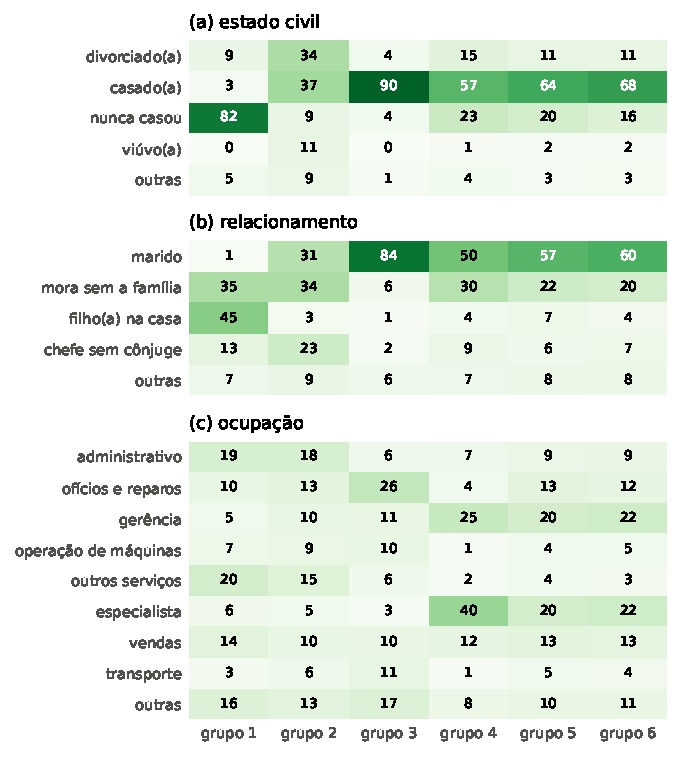
\includegraphics[width=.8\textwidth]{figures/clusters_proporcoes.pdf}
\caption{Composição dos grupos ($k = 6$, seed 42), em \% das pessoas de cada grupo: categorias com pelo menos 10\% em algum grupo; as demais somadas em ``outras''.}
\label{fig:cl_prop}
\end{figure}

A silhueta média, \clSilSeis, esconde diferenças grandes entre os grupos (Figura~\ref{fig:cl_sil}). Os grupos do capital são os mais bem definidos, com silhueta média de \clSilGCinco{} (perda) e \clSilGSeis{} (ganho) e quase nenhuma pessoa com silhueta negativa. Entre os grupos sem capital, os jovens solteiros (\clSilGUm) e os casados em ofícios manuais (\clSilGTres) são os mais coesos, e os profissionais (\clSilGQuatro) já têm \clSilNegGQuatro\% de pessoas mais perto de outro grupo que do próprio. O grupo 2 é o mais difuso: silhueta média de \clSilGDois, com \clSilNegGDois\% das pessoas do lado negativo. Ele reúne quem não se encaixa nos perfis mais nítidos, e é por isso que só aparece a partir de $k = 6$.

\begin{figure}[ht]
\centering
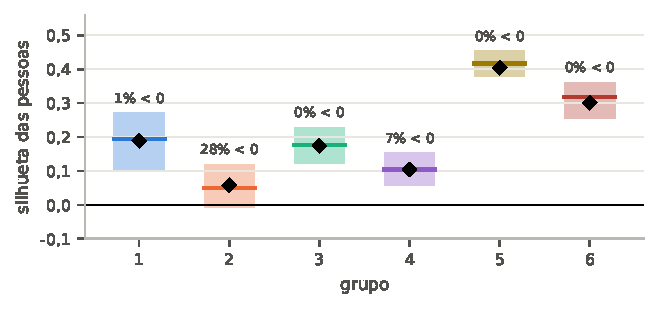
\includegraphics[width=.75\textwidth]{figures/clusters_silhueta.pdf}
\caption{Silhueta das pessoas de cada grupo, na amostra fixa de 10 mil pessoas: a caixa vai do 1º ao 3º quartil, a linha é a mediana, o losango é a média, e o rótulo dá o \% de silhuetas negativas.}
\label{fig:cl_sil}
\end{figure}

A Figura~\ref{fig:cl_pca} projeta as \clColunas{} colunas nas duas direções de maior variância (PCA). A projeção explica só \clVarTotal\% da variância e serve apenas para desenhar, porque o K-means agrupou nas \clColunas{} colunas. Mesmo assim, ela mostra o que as métricas indicaram: os grupos do capital ficam isolados, um em cima e outro embaixo, e os grupos 1 a 4 se encostam numa nuvem contínua, dos jovens solteiros, à esquerda, aos profissionais, à direita.

\begin{figure}[ht]
\centering
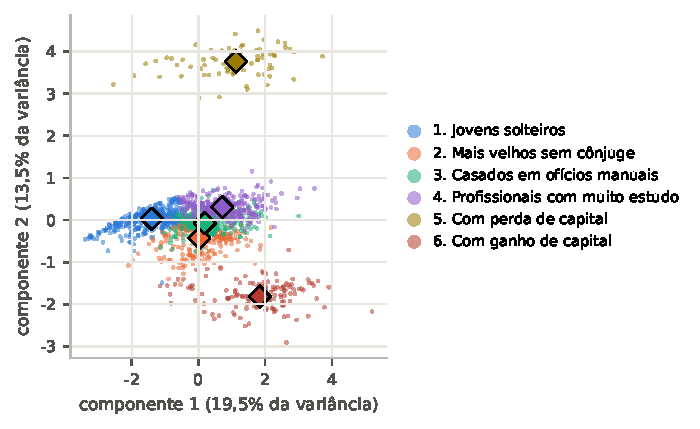
\includegraphics[width=.85\textwidth]{figures/clusters_pca.pdf}
\caption{Os seis grupos nas duas primeiras componentes principais (amostra de 1.500 pessoas); os losangos são os centros dos grupos, calculados com todas as pessoas.}
\label{fig:cl_pca}
\end{figure}

\subsection{Comparação com a renda}\label{sec:cl_renda}

O K-means não viu a renda, e mesmo assim os grupos se ordenam por ela (Figura~\ref{fig:cl_renda}): \clPosUm\% dos jovens solteiros ganham mais de 50 mil, contra \clPosQuatro\% dos profissionais com muito estudo e \clPosSeis\% de quem tem ganho de capital (\clPositivos\% na base inteira). Os atributos que formam os grupos, como idade, estudo, estado civil, ocupação e capital, são os mesmos que explicam a renda.

\begin{figure}[ht]
\centering
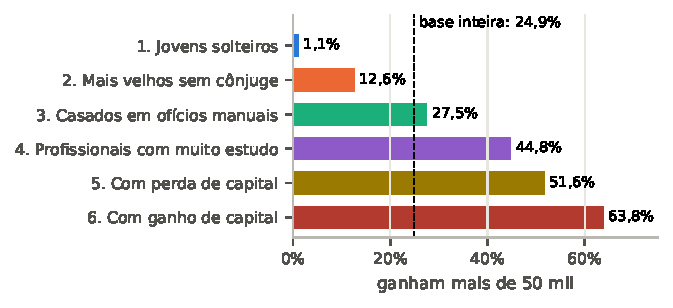
\includegraphics[width=.75\textwidth]{figures/clusters_renda.pdf}
\caption{Percentual de pessoas acima de 50 mil em cada grupo ($k = 6$, seed 42).}
\label{fig:cl_renda}
\end{figure}

Como previsão, porém, os grupos são fracos. Se cada grupo respondesse a renda da sua maioria (os grupos 1 a 4, ``até 50 mil''; os grupos 5 e 6, ``acima''), acertaria \clPureza\% das pessoas, a \emph{pureza} da partição. Responder ``até 50 mil'' para todos já acerta \clChute\%, só \clPurezaGanho{} pontos a menos, e a SVM com kernel RBF, treinada com a renda na parte anterior do trabalho, acerta \clSvmAcc\% no teste (média de 10 divisões). Nenhum grupo é puro: no grupo 4, a chance de renda alta é de \clPosQuatro\%, quase a de uma moeda. O ARI entre os grupos e as duas classes de renda é de \clAriRenda, perto do acaso; com seis grupos e duas classes, ele não chegaria a 1 nem com grupos puros, e por isso a pureza é a métrica mais fácil de ler. O K-means junta pessoas parecidas em todos os atributos, com o mesmo peso para os que importam muito e os que importam pouco para a renda; um classificador aprende com a renda onde fica a fronteira. Os grupos servem para descrever a população, e não para prever a renda de uma pessoa.

\subsection{Raça e sexo nos grupos}\label{sec:cl_sensiveis}

Raça e sexo ficaram fora do agrupamento, como ficaram fora da classificação na parte anterior do trabalho, porque não queremos que o perfil de uma pessoa seja definido por eles. Usamos os dois só depois, para ver como se distribuem nos grupos formados pelos outros atributos (Tabela~\ref{tab:cl_sensiveis}). Por decisão do grupo, essa análise aparece só neste relatório e não nos slides: em uma apresentação curta, os números ficariam sem o contexto que os explica e poderiam ser lidos como uma afirmação sobre pessoas, quando dizem respeito à forma como a base e os atributos foram construídos.

\begin{table}[ht]
\centering
\caption{Sexo e raça em cada grupo ($k = 6$, seed 42), em \% das pessoas do grupo. Nenhum dos dois entrou no agrupamento.}
\label{tab:cl_sensiveis}
\footnotesize
\begin{tabular}{lrrrrrrr}
\toprule
(\%) & Grupo 1 & Grupo 2 & Grupo 3 & Grupo 4 & Grupo 5 & Grupo 6 & Base \\
\midrule
Mulheres & 47,7 & 48,3 & 8,3 & 29,2 & 23,6 & 21,8 & 32,4 \\
\midrule
\multicolumn{8}{l}{\emph{Raça}} \\
Branca & 81,9 & 82,7 & 89,5 & 88,6 & 89,8 & 89,4 & 86,0 \\
Negra & 12,8 & 13,4 & 6,6 & 5,7 & 6,2 & 6,4 & 9,3 \\
Asiática ou do Pacífico & 3,1 & 2,3 & 1,9 & 4,7 & 3,1 & 2,8 & 3,0 \\
Indígena ou esquimó & 1,1 & 1,0 & 1,1 & 0,5 & 0,4 & 0,9 & 0,9 \\
Outra & 1,1 & 0,6 & 0,9 & 0,5 & 0,5 & 0,4 & 0,8 \\
\bottomrule
\end{tabular}

\end{table}

Mesmo fora do agrupamento, os dois se distribuem de forma desigual. O grupo 3 tem só \clMulheresTres\% de mulheres, porque ``marido'', o relacionamento de 84\% do grupo, indica o sexo quase sem exceção. Os grupos 1 e 2, os de menor renda, têm \clMulheresUm\% e \clMulheresDois\% de mulheres (\clMulheresBase\% na base) e a maior proporção de pessoas negras (\clNegrosUm\% e \clNegrosDois\%, contra \clNegrosBase\% na base). Atributos como estado civil, relacionamento e ocupação carregam essa informação, e os grupos a refletem: tirar raça e sexo da entrada não os tira do resultado.

\subsection{Custo}\label{sec:cl_custo}

Cada iteração do K-means custa proporcionalmente ao número de pessoas, ao número de grupos e ao de colunas, e o custo total cresce linearmente com a base. Um ajuste com $k = 6$ e 10 inicializações leva \clTempoSeis{} s nas \clLinhas{} pessoas, num núcleo (\clTempoSeisUm{} s com uma inicialização), e o estudo inteiro, com \clAjustes{} ajustes, cerca de 4 minutos. A Figura~\ref{fig:cl_tempo} mostra o tempo por $k$: ele cresce de \clTempoDois{} s em $k = 2$ para cerca de 1 s de $k = 5$ em diante, acompanhando o número de iterações até a partição parar de mudar (de \clIterDois{} em $k = 2$ para \clIterSeis{} em $k = 6$ e \clIterDez{} em $k = 10$). Com mais grupos, há mais fronteiras a ajustar, e os centros levam mais passos para se acomodar. Com uma só inicialização, o custo cai para cerca de um décimo, mas a resposta muda de uma seed para outra (Seção~\ref{sec:cl_k}).

\begin{figure}[ht]
\centering
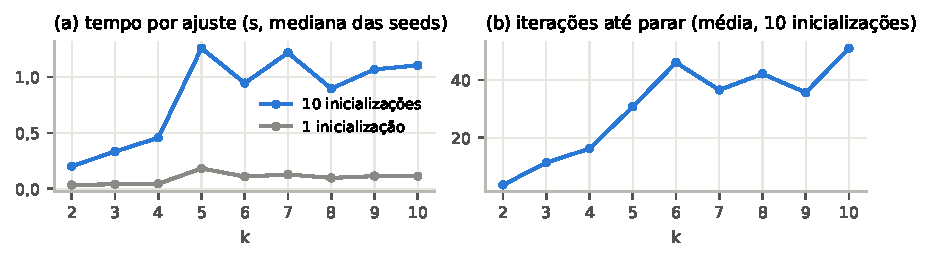
\includegraphics[width=\textwidth]{figures/clusters_tempo.pdf}
\caption{Custo do K-means por $k$, num único núcleo, nas \clLinhas{} pessoas: tempo por ajuste (mediana das 10 seeds) e número médio de iterações.}
\label{fig:cl_tempo}
\end{figure}

\section{Limitações}\label{sec:km_limitacoes}

Os grupos dependem das escolhas que definem a distância. O one-hot, a padronização e o logaritmo no capital dizem o que é ``parecido'', e outra escolha daria outros grupos; os dois grupos do capital são, em parte, efeito do logaritmo. O K-means foi feito para atributos numéricos, e o one-hot é uma adaptação: o centro de um grupo tem proporções nas colunas de texto, e não uma pessoa possível.

A escolha de $k = 6$ combina métricas e interpretação, e $k = 5$ ou $k = 8$ também seriam defensáveis. A silhueta foi calculada numa amostra de 10 mil pessoas. Só o K-means foi testado: algoritmos que não supõem grupos arredondados, ou que dão a cada pessoa uma probabilidade de pertencer a cada grupo, poderiam encontrar outra estrutura.

Deixar raça e sexo fora do agrupamento não impede que os grupos reflitam essas características, porque outros atributos carregam a mesma informação (Seção~\ref{sec:cl_sensiveis}). A curadoria removeu as linhas com valor ausente, e os grupos não descrevem essas pessoas. A base é de 1994, e os perfis valem para aquela população.

\section{Conclusão e trabalhos futuros}

Sem a renda, o K-means dividiu as \clLinhas{} pessoas da base Adult em seis grupos estáveis entre seeds (ARI de \clAriSeis): quatro separados pela fase da vida e pelo tipo de trabalho (jovens solteiros, mais velhos sem cônjuge, casados em ofícios manuais e profissionais com muito estudo) e dois pelo capital. A base, porém, não tem grupos nítidos: a silhueta é de \clSilSeis, e os grupos sem capital são regiões de uma nuvem contínua, das quais a dos mais velhos sem cônjuge é a menos coesa.

O estudo mostrou que o pré-processamento decide os grupos. Com o one-hot, trocar de ocupação afasta duas pessoas tanto quanto \clTrocaAnos{} anos de idade, e as categorias marcam as fronteiras entre os grupos. O logaritmo no capital tira um grupo artificial, formado pelas \clTeto{} pessoas no teto do censo, mas faz quem tem capital formar dois grupos próprios. Mostrou também que as métricas internas sozinhas não escolhem o $k$, e que a estabilidade entre seeds, que exige várias inicializações, ajuda a decidir.

Os grupos se ordenam pela renda, de \clPosUm\% a \clPosSeis\% acima de 50 mil, porque os atributos que os formam são os mesmos que explicam a renda. Como previsão, porém, ficam pouco acima do chute: pureza de \clPureza\%, contra \clChute\%. O K-means serve para descrever a população; para classificar a renda de uma pessoa, um modelo treinado com ela, como a SVM da parte anterior do trabalho (\clSvmAcc\%), é muito melhor.

Os próximos passos seriam usar uma distância própria para dados mistos, como a do k-prototypes, que trata as categorias sem one-hot; representar o capital só como ``tem ou não tem'', para que ele não ocupe dois grupos; e testar uma mistura de gaussianas, que dá a cada pessoa uma probabilidade de pertencer a cada grupo.


\bibliographystyle{sbc}
\bibliography{refs}

\end{document}
